\newpage
\fancyfoot[LO,RE]{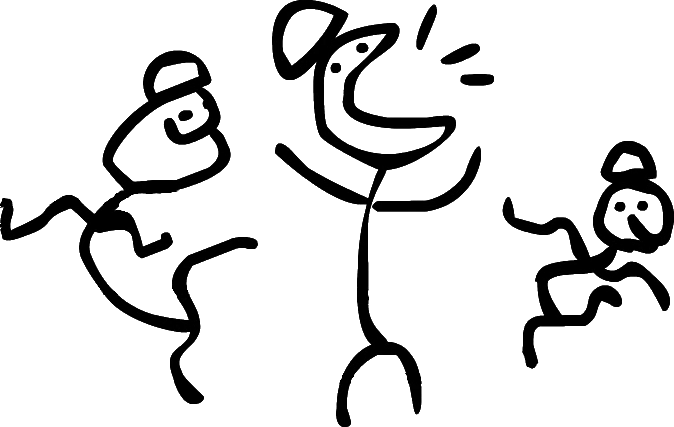
\includegraphics[height=45pt]{images/hutnicy.png}}
\begin{song}{title={Piosenka o hucie}, lyrics={Jakub \say{Dem3000} Dębski}, music={Romek Buga}}
    \begin{intro}
        \say{Czasami w hu^{Ebmaj7}cie spotykamy się wszyscy i pracujemy tam \\
        A ^{f7}czasami nie, czasami śpiewamy piosenki, na przykład moją ulubio-- \\
        Moją ^{B7}ulubioną piosenkę} --- pomyślał sobie, przypomniał sobie swoją ulubioną piosenkę:
    \end{intro}
    \begin{chorus}
        ^{Ebmaj7}Hej! ^*{c7} Otrzymy ^{f7}wanie me^{B7}tali \\
        Z r^{Ebmaj7}ud i z^{c7}łomu ^{f7} ^{B7} \\
        To jest ^{Ebmaj7}to, co ^{c7}lubię naj^{f7}bardziej ^{B7} \\
        To jest ^{Ebmaj7}to, co ^{c7}lubię naj^{f7}bardziej \\
        ^{B7}Wytapiać sz^{Ebmaj7}kło --- i prze^{c7}twarzać produkty sz^{f7}klane ^{B7} \\
        Praca w ^*{Ebmaj7}hu--- ^*{c7}uc ^{f7}ie ^{B7} \\
        Praca w hu^{Ebmaj7}cie
    \end{chorus}
\end{song}

